% 15-418/618 Fall 2026 -- Project Proposal
%
% Build:  latexmk -pdf proposal.tex
%
% NOTE before publishing: do not paste numbers from the UnieAI / 15-712 UMA
% reports (interference ratios, Gemma/Qwen throughput) into this document or
% the public web page. Every such spot is marked \todo.

\documentclass[11pt]{article}
\usepackage[margin=1in]{geometry}
\usepackage[T1]{fontenc}
\usepackage{lmodern}
\usepackage{xcolor}
\usepackage{booktabs}
\usepackage{longtable}
\usepackage{array}
\usepackage{enumitem}
\usepackage{amsmath}
\usepackage{graphicx}
\usepackage[hidelinks]{hyperref}
\usepackage{microtype}
\usepackage{tikz}

\setlist{nosep}
\newcommand{\todo}[1]{\textcolor{red}{\textbf{[TODO: #1]}}}
\newcommand{\code}[1]{\texttt{#1}}
% timeline block: [style]{x0}{x1}{y}{label}{fill}
\newcommand{\blk}[6][]{%
  \draw[fill=#6,#1] (#2,#4) rectangle (#3,#4+0.4);
  \node at ({(#2+#3)/2},#4+0.2) {\scriptsize #5};}

\title{Scheduling Concurrent Coding Agents on\\
  Unified-Memory Hardware\\[6pt]
  \large 15-418/618 Fall 2026 Project Proposal}
\author{Jerry Chen (chinjuic) \and Ethan Chiu (ethanchi)}
\date{November 9, 2026}

\begin{document}
\maketitle

% ---------------------------------------------------------------------------
\section*{URL}
Project page: \url{https://kogby.github.io/pp-final-project/}\\
Code: \url{https://github.com/kogby/pp-final-project}

% ---------------------------------------------------------------------------
\section*{Summary}
We will parallelize the sequential loop of a coding agent (LLM generation
$\rightarrow$ tool execution $\rightarrow\cdots$) on two unified-memory machines (NVIDIA DGX Spark \& M5 Mackbook Pro).
We work at two levels: (1) within one agent, we overlap CPU-side tool execution with GPU-side generation through pipelining and through speculation on the next tool call or its result; (2) across agents, we run several independent agent sessions on one machine with a shared, batched decode stream and concurrent tools. We expect most of the benefit coming from the second level with an estimation from public traces.
We plan to replay real agent traces on \code{llama.cpp} and run tool calls as real programs (e.g., \code{pytest}, \code{pandas}).
Our central questions are (1) how much parallelization gains on a machine where the extra work shares memory bandwidth and capacity with the critical path, and (2) how much a scheduler gains when it knows each tool's and agent's workload.


% ---------------------------------------------------------------------------
\section*{Background}

\paragraph{The sequential agent loop.}
A coding agent (Claude Code, Codex, \ldots) runs in a loop. the LLM generates a response that ends in one or more tool calls, then the harness executes the tools, whose output is appended to the context and the LLM generates again. 
Each LLM step depends on the previous tool result, and each tool call
depends on the previous LLM step, so one request is a long dependency chain.
\\
\\
Public traces of real coding-agent sessions (e.g. TraceLab~\cite{tracelab}: 357k LLM rounds, 433k tool calls from 43 users) show roughly 8.8 LLM steps and 10.8 tool calls per user request. Tool latency is heavy-tailed that about 4\% of calls that run over a minute account for about 85\% of tool time.

\paragraph{Four potential ways to speed up one agent.} (Figure~\ref{fig:spec}):
\begin{itemize}
  \item Pipelining (Conveyor~\cite{conveyor}):
    start executing a tool call as soon as its arguments have been decoded,while the LLM is still generating the rest of its response.
  \item Speculation (PASTE~\cite{paste}):
    predict the next tool call from the pattern of previous calls and execute it during generation. (discard result if no match)
  \item DAG decomposition (LLMCompiler~\cite{llmcompiler}):
    execute independent tool calls concurrently.
  \item Result speculation (value prediction~\cite{lipasti}):
    while a tool runs, fork $k$ generation branches, each conditioned on a
    likely tool outcome (e.g., build succeeds / fails). When the tool finishes, only keep the branch with correct assumed value.
\end{itemize}


PASTE and Conveyor hide tool or generation latency behind each other by speculation. All four ways above trade extra work
for a potential shorter excution time. Prior systems evaluate on discrete GPUs, while extra work on CPU and DRAM are basically considered free. But that's not the case in a unified memory system.


\begin{figure}[h]
\centering
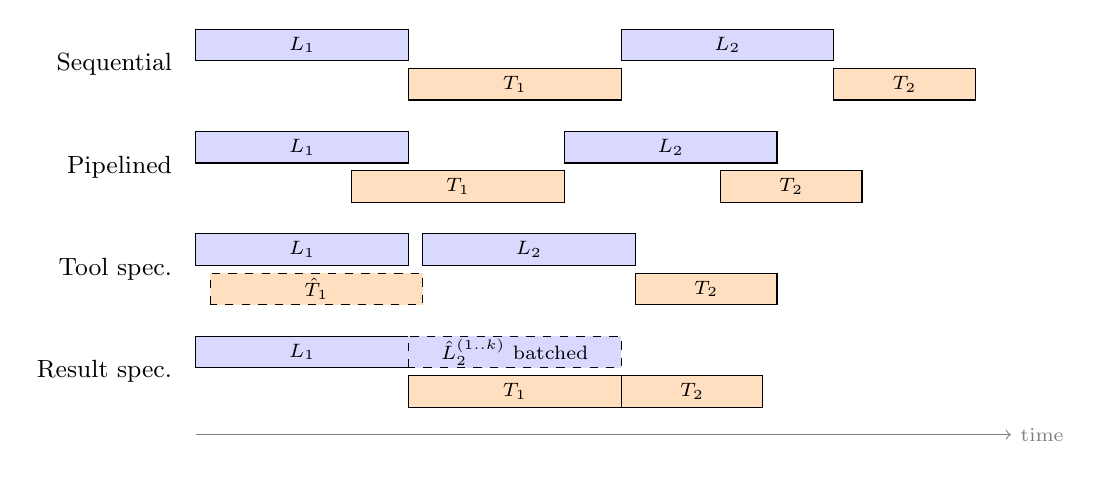
\begin{tikzpicture}[x=0.9cm,y=1cm]
  % Sequential
  \node[left] at (-0.2,-0.05) {\small Sequential};
  \blk{0}{3}{0}{$L_1$}{blue!15}   \blk{6}{9}{0}{$L_2$}{blue!15}
  \blk{3}{6}{-0.5}{$T_1$}{orange!25} \blk{9}{11}{-0.5}{$T_2$}{orange!25}
  % Pipelined
  \node[left] at (-0.2,-1.35) {\small Pipelined};
  \blk{0}{3}{-1.3}{$L_1$}{blue!15} \blk{5.2}{8.2}{-1.3}{$L_2$}{blue!15}
  \blk{2.2}{5.2}{-1.8}{$T_1$}{orange!25} \blk{7.4}{9.4}{-1.8}{$T_2$}{orange!25}
  % Tool speculation
  \node[left] at (-0.2,-2.65) {\small Tool spec.};
  \blk{0}{3}{-2.6}{$L_1$}{blue!15} \blk{3.2}{6.2}{-2.6}{$L_2$}{blue!15}
  \blk[dashed]{0.2}{3.2}{-3.1}{$\hat T_1$}{orange!25}
  \blk{6.2}{8.2}{-3.1}{$T_2$}{orange!25}
  % Result speculation
  \node[left] at (-0.2,-3.95) {\small Result spec.};
  \blk{0}{3}{-3.9}{$L_1$}{blue!15}
  \blk[dashed]{3}{6}{-3.9}{$\hat L_2^{(1..k)}$ batched}{blue!15}
  \blk{3}{6}{-4.4}{$T_1$}{orange!25} \blk{6}{8}{-4.4}{$T_2$}{orange!25}
  \draw[->,gray] (0,-4.75) -- (11.5,-4.75) node[right]{\scriptsize time};
\end{tikzpicture}
\caption{One agent under four schedules. The L lane is decode and the T lane is tool execution.}
\label{fig:spec}
\end{figure}




\paragraph{Estimate how much speedup one agent can gain.}
At step $i$, overlap can hide at most $\min(L_i, T_i)$, where $L_i$ is the
LLM time and $T_i$ the tool time, so the possible headroom of a request and the best speedup are
\[
  H \;=\; \frac{\sum_i \min(L_i, T_i)}{\sum_i (L_i + T_i)}, \qquad
  \text{speedup} \;\le\; \frac{1}{1 - H}.
\]
We computed $H$ over 82k TraceLab requests, with $L_i$ from recorded cloud times or local times measured on the M5~Pro(Table~\ref{tab:headroom}). 
We found that tool time concentrates in a few long calls and 40\% of requests call no tool at all.
With one-step overlap, a single agent gains at most $1.05$--$1.07\times$, and up to $1.20\times$ if speculation could look arbitrarily far ahead.
Overlap inside one agent has a ceiling.


\begin{table}[h]
\centering\small
\begin{tabular}{@{}llrrrrr@{}}
\toprule
LLM time & Context & Tool share & $H$ (one step) & Bound
  & $H$ (unlimited) & Bound \\
\midrule
Cloud (recorded) & -- & 32\% & 6.5\% & 1.07$\times$ & 16.8\% & 1.20$\times$ \\
Qwen3-8B & 16k & 23\% & 5.9\% & 1.06$\times$ & 15.0\% & 1.18$\times$ \\
Qwen3-8B & 32k & 17\% & 5.2\% & 1.06$\times$ & 12.6\% & 1.14$\times$ \\
Qwen3-8B & 64k & 12\% & 4.4\% & 1.05$\times$ &  9.7\% & 1.11$\times$ \\
\bottomrule
\end{tabular}
\caption{Single-agent headroom over TraceLab. ``Unlimited'' assumes perfect speculation with no lookahead limit.}
\label{tab:headroom}
\end{table}

\paragraph{Many agents on one machine.}
With the limit indicated above, we then looked into running multiple agents on one machine. When several agents run at once, there are no data dependencies across
sessions, which opens up opportunities for parallelism (Figure~\ref{fig:system}). 
The GPU decodes every agent that is currently generating as one batch.
When fewer than $N$ agents are generating, the freed up batch slots can also run speculative work for agents that are waiting on a tool.

\begin{figure}[h]
\centering
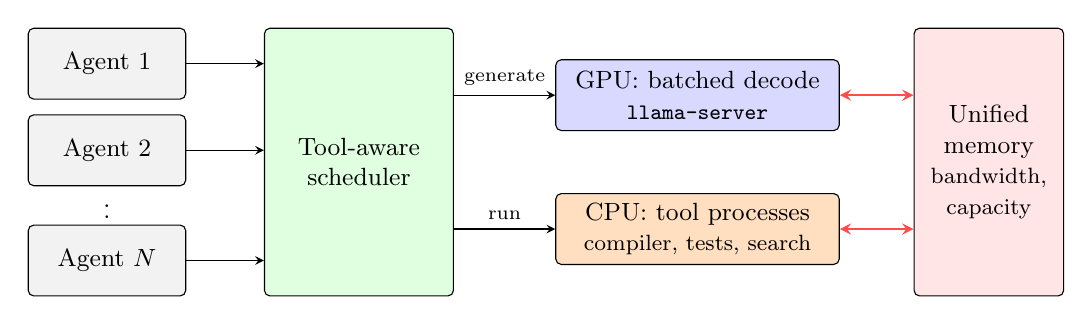
\begin{tikzpicture}[
  box/.style={draw, rounded corners=2pt, align=center, font=\small,
              minimum height=0.9cm},
  >=stealth]
  \node[box, fill=gray!10, minimum width=2cm] (a1) at (0,1.1)  {Agent 1};
  \node[box, fill=gray!10, minimum width=2cm] (a2) at (0,0)    {Agent 2};
  \node[font=\small]                               at (0,-0.75) {$\vdots$};
  \node[box, fill=gray!10, minimum width=2cm] (an) at (0,-1.4) {Agent $N$};
  \node[box, fill=green!12, minimum width=2.4cm, minimum height=3.4cm]
       (sch) at (3.2,-0.15) {Tool-aware\\scheduler};
  \node[box, fill=blue!15, minimum width=3.6cm] (gpu) at (7.5,0.7)
       {GPU: batched decode\\{\footnotesize\code{llama-server}}};
  \node[box, fill=orange!25, minimum width=3.6cm] (cpu) at (7.5,-1.0)
       {CPU: tool processes\\{\footnotesize compiler, tests, search}};
  \node[box, fill=red!10, minimum width=1.9cm, minimum height=3.4cm]
       (mem) at (11.2,-0.15)
       {Unified\\memory\\{\footnotesize bandwidth,}\\{\footnotesize capacity}};
  \foreach \a in {a1,a2,an}
    \draw[->] (\a.east) -- (sch.west |- \a.east);
  \draw[->] (sch.east |- gpu.west) -- node[above,font=\scriptsize]{generate} (gpu.west);
  \draw[->] (sch.east |- cpu.west) -- node[above,font=\scriptsize]{run} (cpu.west);
  \draw[<->, thick, red!70] (gpu.east) -- (mem.west |- gpu.east);
  \draw[<->, thick, red!70] (cpu.east) -- (mem.west |- cpu.east);
\end{tikzpicture}
\caption{System overview. $N$ independent agents share one machine: the GPU
decodes every generating agent in one batch and the CPU runs their tools. Both
draw on the same memory, so the scheduler decides when each tool call runs.}
\label{fig:system}
\end{figure}
 
\paragraph{Related systems.}
EdgeAgent~\cite{edgeagent} schedules several agents on unified memory but simulates tool calls as pauses. it does not measure how generation affects the tools. SERENO~\cite{sereno} studies bandwidth contention between LLM inference and foreground apps on phones.
We run real tools and batched generation locally on the unified memory.



% ---------------------------------------------------------------------------
\section*{The Challenge}

\paragraph{What we hope to learn:}
How many agents can one unified-memory machine run before memory contention stops the gain?
When does parallelizing the agent loop pay off on a machine where the parallel work and the critical path share memory, and what does a scheduler need to know
about each tool to make that decision?

\paragraph{Dependencies.}
Within one agent, the workload is a chain by construction. The LLM must see the tool output before it can decide the next call. The only parallelism available is
speculative (we guess the next call) or partial (we start the
call before the LLM has finished talking), and both have a cost when wrong.
so static scheduling is impossible. The runtime has to decide
whether to speculate and how much.
\\
A wrong speculation must leave no trace, but tools like compilers, test runners, and
\code{pandas} scripts write files. Solving it with isolation has its own setup cost, which must stay below the latency it hides.


\paragraph{Memory access and communication.}
On a unified-memory system, the CPU and GPU share one memory pool. Decoding is bandwidth-bound, since every step streams the weights and every batched agent's KV cache through that memory, and many tools also consume significant bandwidth or cache.
On a discrete GPU the same tool traffic goes to the host's own DRAM and never
touches the GPU's memory.
A running tool therefore slows decoding for the whole batch, and decoding slows every running tool. We did preliminary experiments and found that this relation isn't symmetrically. A basic mitigation is to stagger decode away from tools, but that leaves the GPU idle and costs throughput.

Different tools have different footprints. A good policy
has to know, per tool, how much it hurts decoding and how much decoding hurts
it. We didn't find prior work reports it for agent tools on unified memory.

Agents also interfere with each other. Batching $N$ agents into one decode
stream shares the weight reads, but each agent adds its own KV cache to every
step. With a long agent context, one agent's KV cache can be as large as the
quantized weights, and each added agent slows the step for all the others. Prefill adds a second kind of
interference. When a tool returns, its output (for example, a long test or
build log) is appended to that agent's context and must be prefilled before the
agent can decode again. \code{llama-server} puts this prefill in the same batch
as the other agents' decode steps, so one agent's long tool output slows
everyone's generation. If an agent's KV cache is evicted, its whole context has to be prefilled again.

\paragraph{Divergence.}
Speculative branches behave like divergent lanes. The $k$ branches in a batch
generate different lengths, so the batch runs until its longest branch
finishes or is cancelled. Mispredicted branches are wasted lanes, and a
mispredicted tool speculation is wasted CPU work that still occupies the
memory system.

% ---------------------------------------------------------------------------
\section*{Resources}

\paragraph{Hardware.}
\begin{itemize}
  \item NVIDIA GB10 / DGX Spark (128\,GB unified memory, 273\,GB/s bandwidth, 10P+10E Arm cores, Blackwell GPU, CUDA). 
  \item Apple M5~Pro laptop (24\,GB unified memory, 5P+10E CPU cores, 16-core GPU, Metal).
  \\
  We plan to develop and iterate on M5 Pro laptop, then do several benchmarks on DGX Spark.
\end{itemize}

\paragraph{Software.}
\code{llama.cpp} / \code{llama-server} for inference on both CUDA and Metal. We will write the runtime, simulator, and scheduler in Python. Tools are unmodified programs such as \code{ripgrep}, \code{clang}/\code{gcc}, \code{pytest}, or \code{pandas}. 
For profiling we use tools such as Nsight Systems and \code{perf} on Linux, and \code{time} and Instruments on macOS.

\paragraph{Datasets.}
TraceLab~\cite{tracelab} (public). We may look for more traces if needed.

\paragraph{Starting point.}
We start from scratch for the runtime, simulator, and scheduler, and reuse \code{llama.cpp}.

% ---------------------------------------------------------------------------
\section*{Goals and Deliverables}
 
\paragraph{Baselines.}
\begin{itemize}[leftmargin=4.5em]
  \item[\textbf{Solo}] One agent on the machine: decode and tool call run in order, while independent calls of one step run concurrently. This serves as reference for scaling efficiency.
  \item[\textbf{Naive}] $N$ agents share one \code{llama-server} with
    continuous batching. Every tool runs when issued. This is the baseline we must beat.
  \item[\textbf{Stagger}] A naive mitigation of tool slowdown by adding decoding pauses whenever a tool runs.
  \item[\textbf{Ideal}] We measure each decode step and tool alone, then add up these isolated times along each of the $N$ agents' traces to compute the best achievable time, as if there were no contention between agents and no cost of memory sharing. 
\end{itemize}


\paragraph{Metrics.}
\begin{itemize}
  \item Throughput (agent requests completed per unit time) and per-request active time (time from user prompt to final response), as functions of $N$.
  \item Scaling efficiency: throughput$(N)$ / ($N \times$ throughput$(1)$).
  \item Interference: slowdown of each tool call and of decoding relative to isolated runs.
  \item Recovered gap: (Naive $-$ Our time) / (Naive $-$ Ideal), for throughput and active time.
\end{itemize}


\paragraph{Plan to achieve.}
\begin{enumerate}
  \item \textbf{Workload model} from traces: per-agent tool share, tool
    duration by category, token counts per step, and the single-agent headroom
    $H$. We completed M5~Pro (Table~\ref{tab:headroom}), and we will repeat the
    analysis on GB10.
  \item \textbf{Tool data cards}: a profile of each tool on both machines at different numbers of agents, including metrics like: cores, peak memory, and bandwidth used, how much it slows decoding, and how much decoding slows it.
  \item \textbf{Multi-agent replay runtime}: build the program that replays $N$ recorded agent sessions at once, with real tools and the same token counts as the original sessions, so every scheduling policy is tested on identical, repeatable workloads.
  \item \textbf{Scaling study}: sweep $N$ on both platforms for Naive and
    Stagger and compare against Ideal. Find the bottleneck that stops scaling
    on each machine, whether it is capacity or bandwidth.
  \item \textbf{Tool-aware scheduler}: use what we learn about each tool to
    schedule when tools and generation should run, so that concurrent agents
    interfere less, and compare it against Naive, Stagger, and Ideal.
\end{enumerate}

\paragraph{Targets.}
\begin{itemize}
  \item Recover at least 50\% of the Naive--Ideal gap in p95 active time on the GB10 when the number of agents is greater than a certain number (e.g. $N=8$).
  \item Match Stagger's p95 active time with at least 20\% higher throughput.
    Our scheduler should leave the GPU idle less often than Stagger by
    pausing decoding only for heavy tools to avoid contention, while
    achieving the same latency for each request.
\end{itemize}


\paragraph{Hope to achieve.}
\begin{enumerate}
  \item \textbf{Speculation in the batch slack}. When fewer agents are
    generating, the free batch slots can run speculative work for agents that
    are waiting on a tool. A branch can be committed only if its assumed
    output is exactly the text the harness would append, so common outcomes
    must be canonicalized, and speculative tools must run in an isolated copy
    of the workspace. The accuracy at which speculation breaks even should depend on load.
  \item \textbf{An online version of the policy}. Sense contention from decode
    latency instead of relying on data cards.
\end{enumerate}
 
\paragraph{If progress is slower:}
\begin{enumerate}
  \item Workload model, tool data cards, the replay runtime, the simulator, and the
    $N$ sweep for Naive and Stagger on both platforms. The deliverable is then the
    characterization: where scaling stops on each machine and why.
  \item If replaying real tools proves unreliable, we replace them with synthetic tools (sleep, CPU
    loop, bandwidth kernel) calibrated to the data cards.
\end{enumerate}
 
\paragraph{Poster.}
We plan to includes plot such as: throughput and p95 active time versus the number of agent on both platforms, 
with the baselines and our scheduling policy measured against Ideal. 
We will also show a timeline of $N$ replayed agents under different scheduling along with live replays on the laptop.
 
% ---------------------------------------------------------------------------
\section*{Platform Choice}
Our question is about machines whose CPU and GPU share memory, so we use two unified-memory machines that cover both vendors and operating systems that ship them. 
They differ by about $5\times$ in memory capacity, so we expect the M5~Pro laptop to run out of KV-cache space first and the GB10 to saturate
bandwidth first.
We use \code{llama.cpp} because it runs on both CUDA and Metal with the same quantized weights, which removes the engine as a variable.
 
\paragraph{Development order.}
We develop and debug on the M5~Pro laptop and use the GB10 mainly as the measurement machine. We check correctness under every policy: a replayed agent should produce the same tool outputs, the same token counts per step, and the same final transcript whether it runs alone or with $N-1$ others. Only timing may differ between runs and platforms.
 
% ---------------------------------------------------------------------------
\section*{Schedule}
 
{\small
\begin{longtable}{@{}p{2.4cm}p{13.6cm}@{}}
\toprule
\textbf{Dates} & \textbf{Goal} \\
\midrule
\endhead
Nov 9--12 & Build the workload model from traces and measure single-agent headroom (done on laptop already). Measure prefill and decode rates versus context length and batch size. \\
Nov 13--15 & Profile how each tool uses cores, memory, and bandwidth, alone and concurrent with batched generation. \\
Nov 16--19 & Build the multi-agent runtime and check that every agent's transcript is identical alone and in a group. \\
Nov 20--22 & Build the ideal baseline and validate it at $N = 1$. Write the milestone report. \\
\textbf{Nov 23} & \textbf{Milestone report due.} \\
Nov 23--26 & Profile the tools on the GB10. Sweep $N$ with naive concurrency on both machines. \\
Nov 27--29 & Add stagger baseline. Measure the gap to the simulator on each machine and profile it. \\
Nov 30--Dec 2 & Build and refine the policy. \\
Dec 3--5 & Add the limit on how many agents could run at once and the core placement on the GB10. Compare the policy against Naive, Stagger, and Ideal. \\
Dec 6--8 & Buffer time or time for extra goals.
\\
Dec 9--10 & Write the final report. \\
\textbf{Dec 10} & \textbf{Final report due.} \\
\textbf{Dec 11} & \textbf{Poster session.} \\
\bottomrule
\end{longtable}}
 
% ---------------------------------------------------------------------------
{\small
\bibliographystyle{unsrt}
\bibliography{refs}}
 
\end{document}
